% =====================================================================
%  appendix_robustness.tex
%  Supplementary appendix for amr_complexity.tex.
%
%  Include it just before \end{document} in the main paper with
%        % =====================================================================
%  appendix_robustness.tex
%  Supplementary appendix for amr_complexity.tex.
%
%  Include it just before \end{document} in the main paper with
%        % =====================================================================
%  appendix_robustness.tex
%  Supplementary appendix for amr_complexity.tex.
%
%  Include it just before \end{document} in the main paper with
%        % =====================================================================
%  appendix_robustness.tex
%  Supplementary appendix for amr_complexity.tex.
%
%  Include it just before \end{document} in the main paper with
%        \input{appendix_robustness}
%  It reuses the main file's macros (\rca, \N, \I, \num) and the
%  booktabs / siunitx packages already loaded there.  The \providecommand
%  guards below let it also compile on its own if needed.
% =====================================================================
\providecommand{\rca}{\mathrm{RCA}}
\providecommand{\N}{\mathcal{N}}
\providecommand{\I}{\mathcal{I}}

\appendix

% ---------------------------------------------------------------------
\section{Robustness to the minimum-isolate threshold}
\label{app:minN}
% ---------------------------------------------------------------------
Every quantity in the paper is built from the pooled resistance-fraction matrix, in which a
species--antibiotic cell is retained only if it is supported by at least $n_{\min}$ tested isolates
in the pooling window. Throughout the main text we use $n_{\min}=30$: below this the resistance
fraction $r_{pa}=n_R/n_{\text{tested}}$ is too noisy to binarize reliably, while much above it the
matrix is thinned to the point where the within-block Spearman correlations lose power. To confirm
that no conclusion is an artefact of this single choice, we re-ran the \emph{entire} pipeline
(binarization, spectral co-clustering, nestedness, Fitness--Complexity, external validation and the
rolling-origin forecast) at $n_{\min}\in\{10,30,50\}$.\footnote{The threshold is the only quantity
changed. Note that the summary file distributed with the code
(\texttt{pathogen\_year\_antibiotic\_summary\_minN\_30.csv}) in fact contains \emph{all} cells down
to $n_{\text{tested}}=1$; the effective cut is applied in-code and is what we vary here. The file
name reflects the default rather than a pre-applied filter.}

Table~\ref{tab:minN-structure} reports the structural and external-validation statistics. All of the
paper's qualitative claims are preserved across the whole range: (i) global nestedness $\N$ sits at or
below the degree-preserving null while the in-block nestedness $\I^\ast$ is strongly significant
($z\ge 9.9$ everywhere), so nestedness remains a \emph{local}, block-level property with
$\I^\ast/\N$ between $5$ and $10$; (ii) antibiotic resistance complexity correlates positively with the
WHO AWaRe tier at every threshold, most strongly within blocks and within the Gram-negative block;
and (iii) in-block pathogen fitness separates ESKAPEE from non-ESKAPEE organisms with
$p\le 5\times10^{-6}$ throughout, while the corresponding \emph{global} fitness stays uninformative
(negative correlation with WHO priority), exactly the degeneracy the block analysis is meant to
expose. The AWaRe correlations peak at $n_{\min}=30$: relaxing to $10$ admits noisy low-count cells
that dilute them slightly, whereas tightening to $50$ removes enough antibiotics and species to cost
Spearman power (overall $\rho$ falls from $0.47$ to $0.35$). The default is thus a sensible optimum,
not a fragile edge.

\begin{table}[htbp]
\centering
\caption{Sensitivity of the structural and external-validation results to the minimum-isolate
threshold $n_{\min}$. The pooled window (2015--2024) and all other settings are held fixed;
$z$-scores are against \num{100} degree-preserving randomisations. Every conclusion in the main text
holds across the range; $n_{\min}=30$ (used in the paper) maximises the AWaRe correlations.}
\label{tab:minN-structure}
\small
\begin{tabular}{l ccc}
\toprule
 & \multicolumn{3}{c}{minimum isolates $n_{\min}$} \\
\cmidrule(lr){2-4}
Quantity & $10$ & $30$ (paper) & $50$ \\
\midrule
Resistant cells in $M$ (base rate)          & 191 (0.084) & 131 (0.071) & 99 (0.060) \\
\addlinespace[2pt]
Global nestedness $\N$ ($z$)                 & 0.073 ($-2.1$) & 0.050 ($-4.3$) & 0.039 ($-4.9$) \\
In-block nestedness $\I^\ast$ ($z$)          & 0.384 ($11.6$) & 0.386 ($10.5$) & 0.374 ($9.9$) \\
Ratio $\I^\ast/\N$                           & 5.3 & 7.8 & 9.6 \\
\addlinespace[2pt]
Complexity vs.\ AWaRe, overall $\rho$        & 0.434 & \textbf{0.467} & 0.347 \\
Complexity vs.\ AWaRe, in-block $\rho$       & 0.547 & \textbf{0.590} & 0.442 \\
Complexity vs.\ AWaRe, Gram-neg.\ $\rho$     & 0.613 & \textbf{0.624} & 0.546 \\
\addlinespace[2pt]
Global fitness vs.\ WHO priority $\rho$      & $-0.13$ & $-0.24$ & $-0.22$ \\
In-block fitness, ESKAPEE vs.\ non (median)  & $1.30$ / $-0.41$ & $1.04$ / $-0.39$ & $1.04$ / $-0.19$ \\
In-block fitness, ESKAPEE vs.\ non ($p$, MWU)& $2.4\times10^{-7}$ & $4.6\times10^{-6}$ & $5.6\times10^{-7}$ \\
\bottomrule
\end{tabular}
\end{table}

Table~\ref{tab:minN-forecast} shows the same insensitivity for the headline rolling-origin forecast
(2020--2024). The network-exposure score $\rho_{abx}$ beats the resistance-prevalence baseline at
every threshold. The forecast is essentially unchanged between $n_{\min}=30$ and $50$
(AUC $0.708$ vs.\ $0.702$); only the permissive $n_{\min}=10$ setting degrades it appreciably
(AUC $0.638$), because the extra low-count cells inject label noise into exactly the pairs the
predictor is scored on. The prevalence baseline stays near chance throughout, confirming that the
predictive signal comes from network structure rather than from base rates.

\begin{table}[htbp]
\centering
\caption{Sensitivity of the pooled rolling-origin forecast (origins $2019\ldots2023$, predicting
$2020\ldots2024$) to $n_{\min}$. AUC is the rank-based area under the ROC on the pooled candidate set;
the co-resistance exposure $\rho_{abx}$ dominates the prevalence baseline at every threshold.}
\label{tab:minN-forecast}
\small
\begin{tabular}{l ccc}
\toprule
 & \multicolumn{3}{c}{minimum isolates $n_{\min}$} \\
\cmidrule(lr){2-4}
 & $10$ & $30$ (paper) & $50$ \\
\midrule
Candidate pairs (positives)               & 2274 (191) & 1839 (131) & 1656 (99) \\
Base rate                                 & 0.084 & 0.071 & 0.060 \\
\addlinespace[2pt]
AUC, antibiotic-net $\rho_{abx}$          & 0.638 & \textbf{0.708} & 0.702 \\
AUC, pathogen-net $\rho_{path}$           & 0.622 & 0.628 & 0.593 \\
AUC, prevalence baseline                  & 0.544 & 0.512 & 0.504 \\
\bottomrule
\end{tabular}
\end{table}

% ---------------------------------------------------------------------
\section{Multi-year (multi-horizon) forecasting}
\label{app:horizon}
% ---------------------------------------------------------------------
The rolling-origin test in the main text always predicts one year ahead ($t\to t+1$). A natural
question is how far into the future the co-resistance signal reaches. To isolate the pure effect of
forecast \emph{distance} we fix a single training cutoff $t_0=2019$, build the binary matrix, the
co-resistance projection $W$ and every exposure feature $\rho_{pa}$ \emph{once} from data with
year $\le t_0$, and then score that one frozen model against each future target year $t_0+N$ for
$N=1,\ldots,5$ (i.e.\ 2020 through 2024). The training history, the network and the candidate set are
identical for every horizon; only the target year moves, so any change in AUC is attributable to
forecast distance alone and not to a re-fitted model.

We additionally require that a candidate pathogen--antibiotic pair be \emph{actually tested}
($n_{\text{tested}}\ge n_{\min}$) in the future target year: a predicted pair with no measurement in
$t_0+N$ has no ground truth and is dropped rather than silently counted as a negative. About two
thirds of the frozen candidate set is dropped this way at each horizon (roughly $35\%$ retained),
which is reported alongside the AUC so the shrinking evaluable sample is explicit.

Table~\ref{tab:horizon} gives the result at the paper's $n_{\min}=30$ and is plotted in
Fig.~\ref{fig:horizon}. The striking finding is that predictability does \emph{not} decay with
horizon over this window: the antibiotic-network exposure holds an AUC of $0.68$--$0.74$ all the way
out to five years, with no monotone fall-off, while the prevalence baseline hovers near chance
($0.41$--$0.58$) at every distance. In other words, the structural co-resistance signal identified in
the main text is not a short-lived, next-year-only effect; the pairs a pathogen is network-``exposed''
to remain the pairs it tends to acquire years later. The pathogen-network score $\rho_{path}$ is
weaker and noisier at long range (falling toward $0.5$ by $N=3$), consistent with the main-text
finding that the antibiotic-side projection carries most of the predictive information.

\begin{table}[htbp]
\centering
\caption{Single-cutoff multi-horizon forecast, trained once on $2004$--$2019$ and evaluated on each
future year, restricted to pairs tested in that year ($n_{\min}=30$). Predictability is roughly flat
out to five years; the prevalence baseline stays near chance throughout.}
\label{tab:horizon}
\small
\begin{tabular}{c c cc ccc}
\toprule
Horizon $N$ & Target & Tested pairs & Positives (rate) & AUC $\rho_{abx}$ & AUC $\rho_{path}$ & AUC prevalence \\
\midrule
1 & 2020 & 308 & 22 (0.071) & 0.723 & 0.685 & 0.566 \\
2 & 2021 & 281 & 24 (0.085) & 0.698 & 0.661 & 0.554 \\
3 & 2022 & 298 & 22 (0.074) & 0.681 & 0.508 & 0.407 \\
4 & 2023 & 301 & 19 (0.063) & 0.685 & 0.640 & 0.580 \\
5 & 2024 & 298 & 22 (0.074) & 0.742 & 0.561 & 0.477 \\
\bottomrule
\end{tabular}
\end{table}

\begin{figure}[htbp]
\centering
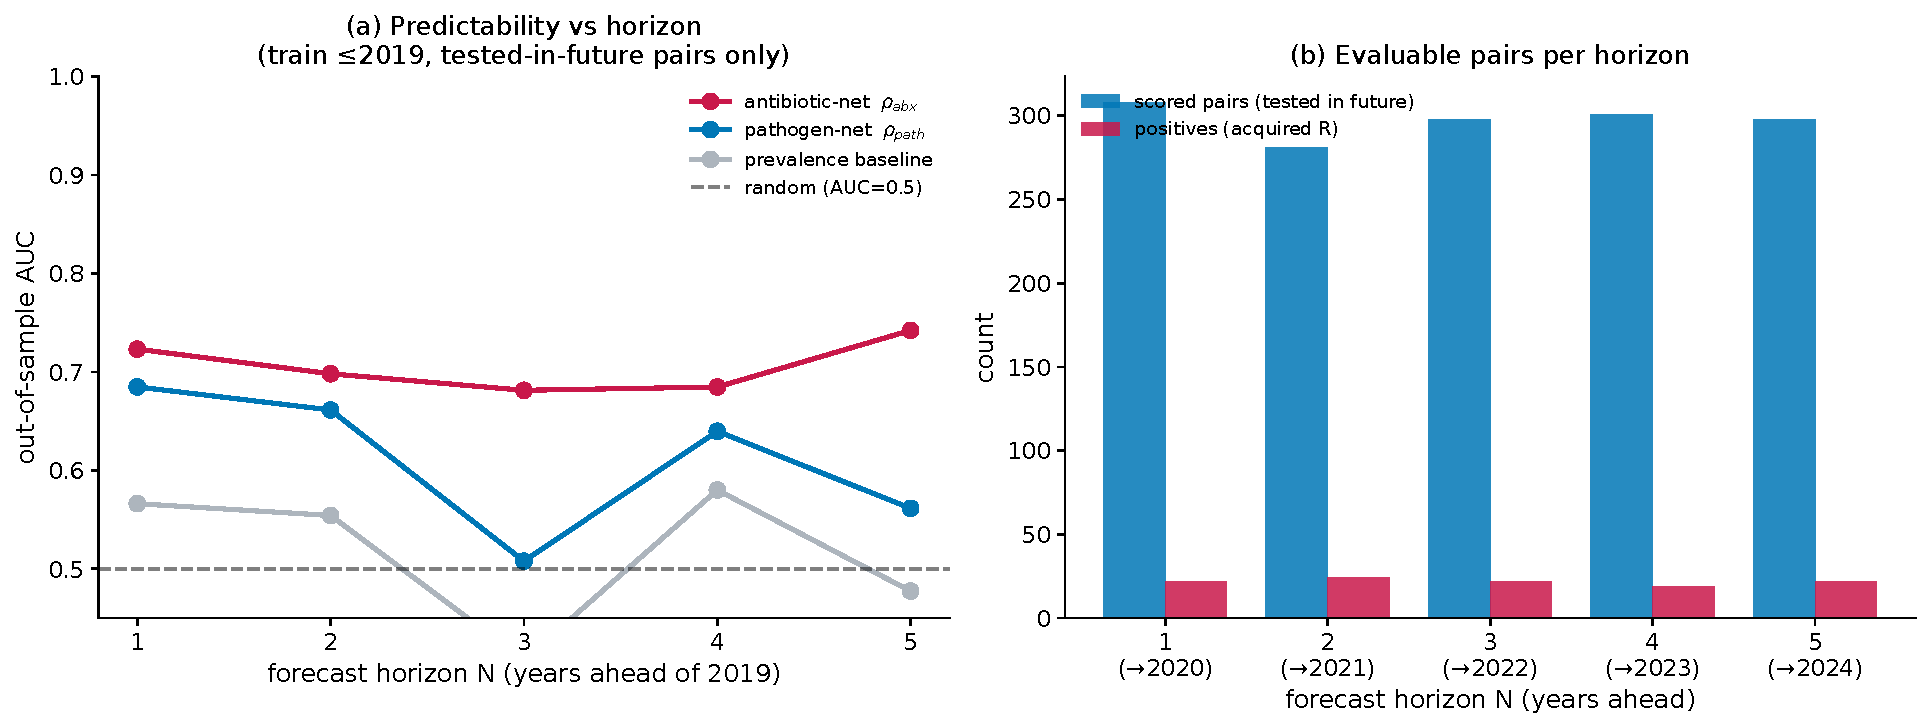
\includegraphics[width=\linewidth]{figures/fig6_horizon}
\caption{Multi-horizon forecasting from a single $t_0=2019$ cutoff. \textbf{(a)} Out-of-sample AUC
versus forecast horizon $N$: the antibiotic-network exposure $\rho_{abx}$ (red) stays at
$\sim\!0.7$ out to five years, well above the prevalence baseline (grey, near $0.5$), while the
pathogen-network score $\rho_{path}$ (blue) decays faster. \textbf{(b)} Number of evaluable pairs and
of realised positives per horizon, after dropping pairs untested in the target year.}
\label{fig:horizon}
\end{figure}

Finally, the horizon result is itself robust to the isolate threshold.
Table~\ref{tab:horizon-minN} repeats the multi-horizon sweep at $n_{\min}\in\{10,30,50\}$: the
antibiotic-network AUC averages $0.66$, $0.71$ and $0.72$ across the five horizons respectively, with
no systematic decay at any threshold. As in Appendix~\ref{app:minN}, the only visible effect is the
mild dilution of the signal at the permissive $n_{\min}=10$ setting; the paper's $n_{\min}=30$ and the
stricter $n_{\min}=50$ give essentially the same multi-year forecast.

\begin{table}[htbp]
\centering
\caption{Robustness of the multi-horizon forecast to $n_{\min}$: out-of-sample AUC of the
antibiotic-network exposure $\rho_{abx}$ at each horizon $N$ (train $\le 2019$). Predictability is flat
in $N$ at every threshold; the bottom row is the across-horizon mean.}
\label{tab:horizon-minN}
\small
\begin{tabular}{c ccc}
\toprule
 & \multicolumn{3}{c}{minimum isolates $n_{\min}$} \\
\cmidrule(lr){2-4}
Horizon $N$ (target) & $10$ & $30$ (paper) & $50$ \\
\midrule
1 (2020) & 0.596 & 0.723 & 0.715 \\
2 (2021) & 0.605 & 0.698 & 0.679 \\
3 (2022) & 0.728 & 0.681 & 0.741 \\
4 (2023) & 0.631 & 0.685 & 0.734 \\
5 (2024) & 0.715 & 0.742 & 0.723 \\
\midrule
mean     & 0.655 & 0.706 & 0.718 \\
\bottomrule
\end{tabular}
\end{table}

%  It reuses the main file's macros (\rca, \N, \I, \num) and the
%  booktabs / siunitx packages already loaded there.  The \providecommand
%  guards below let it also compile on its own if needed.
% =====================================================================
\providecommand{\rca}{\mathrm{RCA}}
\providecommand{\N}{\mathcal{N}}
\providecommand{\I}{\mathcal{I}}

\appendix

% ---------------------------------------------------------------------
\section{Robustness to the minimum-isolate threshold}
\label{app:minN}
% ---------------------------------------------------------------------
Every quantity in the paper is built from the pooled resistance-fraction matrix, in which a
species--antibiotic cell is retained only if it is supported by at least $n_{\min}$ tested isolates
in the pooling window. Throughout the main text we use $n_{\min}=30$: below this the resistance
fraction $r_{pa}=n_R/n_{\text{tested}}$ is too noisy to binarize reliably, while much above it the
matrix is thinned to the point where the within-block Spearman correlations lose power. To confirm
that no conclusion is an artefact of this single choice, we re-ran the \emph{entire} pipeline
(binarization, spectral co-clustering, nestedness, Fitness--Complexity, external validation and the
rolling-origin forecast) at $n_{\min}\in\{10,30,50\}$.\footnote{The threshold is the only quantity
changed. Note that the summary file distributed with the code
(\texttt{pathogen\_year\_antibiotic\_summary\_minN\_30.csv}) in fact contains \emph{all} cells down
to $n_{\text{tested}}=1$; the effective cut is applied in-code and is what we vary here. The file
name reflects the default rather than a pre-applied filter.}

Table~\ref{tab:minN-structure} reports the structural and external-validation statistics. All of the
paper's qualitative claims are preserved across the whole range: (i) global nestedness $\N$ sits at or
below the degree-preserving null while the in-block nestedness $\I^\ast$ is strongly significant
($z\ge 9.9$ everywhere), so nestedness remains a \emph{local}, block-level property with
$\I^\ast/\N$ between $5$ and $10$; (ii) antibiotic resistance complexity correlates positively with the
WHO AWaRe tier at every threshold, most strongly within blocks and within the Gram-negative block;
and (iii) in-block pathogen fitness separates ESKAPEE from non-ESKAPEE organisms with
$p\le 5\times10^{-6}$ throughout, while the corresponding \emph{global} fitness stays uninformative
(negative correlation with WHO priority), exactly the degeneracy the block analysis is meant to
expose. The AWaRe correlations peak at $n_{\min}=30$: relaxing to $10$ admits noisy low-count cells
that dilute them slightly, whereas tightening to $50$ removes enough antibiotics and species to cost
Spearman power (overall $\rho$ falls from $0.47$ to $0.35$). The default is thus a sensible optimum,
not a fragile edge.

\begin{table}[htbp]
\centering
\caption{Sensitivity of the structural and external-validation results to the minimum-isolate
threshold $n_{\min}$. The pooled window (2015--2024) and all other settings are held fixed;
$z$-scores are against \num{100} degree-preserving randomisations. Every conclusion in the main text
holds across the range; $n_{\min}=30$ (used in the paper) maximises the AWaRe correlations.}
\label{tab:minN-structure}
\small
\begin{tabular}{l ccc}
\toprule
 & \multicolumn{3}{c}{minimum isolates $n_{\min}$} \\
\cmidrule(lr){2-4}
Quantity & $10$ & $30$ (paper) & $50$ \\
\midrule
Resistant cells in $M$ (base rate)          & 191 (0.084) & 131 (0.071) & 99 (0.060) \\
\addlinespace[2pt]
Global nestedness $\N$ ($z$)                 & 0.073 ($-2.1$) & 0.050 ($-4.3$) & 0.039 ($-4.9$) \\
In-block nestedness $\I^\ast$ ($z$)          & 0.384 ($11.6$) & 0.386 ($10.5$) & 0.374 ($9.9$) \\
Ratio $\I^\ast/\N$                           & 5.3 & 7.8 & 9.6 \\
\addlinespace[2pt]
Complexity vs.\ AWaRe, overall $\rho$        & 0.434 & \textbf{0.467} & 0.347 \\
Complexity vs.\ AWaRe, in-block $\rho$       & 0.547 & \textbf{0.590} & 0.442 \\
Complexity vs.\ AWaRe, Gram-neg.\ $\rho$     & 0.613 & \textbf{0.624} & 0.546 \\
\addlinespace[2pt]
Global fitness vs.\ WHO priority $\rho$      & $-0.13$ & $-0.24$ & $-0.22$ \\
In-block fitness, ESKAPEE vs.\ non (median)  & $1.30$ / $-0.41$ & $1.04$ / $-0.39$ & $1.04$ / $-0.19$ \\
In-block fitness, ESKAPEE vs.\ non ($p$, MWU)& $2.4\times10^{-7}$ & $4.6\times10^{-6}$ & $5.6\times10^{-7}$ \\
\bottomrule
\end{tabular}
\end{table}

Table~\ref{tab:minN-forecast} shows the same insensitivity for the headline rolling-origin forecast
(2020--2024). The network-exposure score $\rho_{abx}$ beats the resistance-prevalence baseline at
every threshold. The forecast is essentially unchanged between $n_{\min}=30$ and $50$
(AUC $0.708$ vs.\ $0.702$); only the permissive $n_{\min}=10$ setting degrades it appreciably
(AUC $0.638$), because the extra low-count cells inject label noise into exactly the pairs the
predictor is scored on. The prevalence baseline stays near chance throughout, confirming that the
predictive signal comes from network structure rather than from base rates.

\begin{table}[htbp]
\centering
\caption{Sensitivity of the pooled rolling-origin forecast (origins $2019\ldots2023$, predicting
$2020\ldots2024$) to $n_{\min}$. AUC is the rank-based area under the ROC on the pooled candidate set;
the co-resistance exposure $\rho_{abx}$ dominates the prevalence baseline at every threshold.}
\label{tab:minN-forecast}
\small
\begin{tabular}{l ccc}
\toprule
 & \multicolumn{3}{c}{minimum isolates $n_{\min}$} \\
\cmidrule(lr){2-4}
 & $10$ & $30$ (paper) & $50$ \\
\midrule
Candidate pairs (positives)               & 2274 (191) & 1839 (131) & 1656 (99) \\
Base rate                                 & 0.084 & 0.071 & 0.060 \\
\addlinespace[2pt]
AUC, antibiotic-net $\rho_{abx}$          & 0.638 & \textbf{0.708} & 0.702 \\
AUC, pathogen-net $\rho_{path}$           & 0.622 & 0.628 & 0.593 \\
AUC, prevalence baseline                  & 0.544 & 0.512 & 0.504 \\
\bottomrule
\end{tabular}
\end{table}

% ---------------------------------------------------------------------
\section{Multi-year (multi-horizon) forecasting}
\label{app:horizon}
% ---------------------------------------------------------------------
The rolling-origin test in the main text always predicts one year ahead ($t\to t+1$). A natural
question is how far into the future the co-resistance signal reaches. To isolate the pure effect of
forecast \emph{distance} we fix a single training cutoff $t_0=2019$, build the binary matrix, the
co-resistance projection $W$ and every exposure feature $\rho_{pa}$ \emph{once} from data with
year $\le t_0$, and then score that one frozen model against each future target year $t_0+N$ for
$N=1,\ldots,5$ (i.e.\ 2020 through 2024). The training history, the network and the candidate set are
identical for every horizon; only the target year moves, so any change in AUC is attributable to
forecast distance alone and not to a re-fitted model.

We additionally require that a candidate pathogen--antibiotic pair be \emph{actually tested}
($n_{\text{tested}}\ge n_{\min}$) in the future target year: a predicted pair with no measurement in
$t_0+N$ has no ground truth and is dropped rather than silently counted as a negative. About two
thirds of the frozen candidate set is dropped this way at each horizon (roughly $35\%$ retained),
which is reported alongside the AUC so the shrinking evaluable sample is explicit.

Table~\ref{tab:horizon} gives the result at the paper's $n_{\min}=30$ and is plotted in
Fig.~\ref{fig:horizon}. The striking finding is that predictability does \emph{not} decay with
horizon over this window: the antibiotic-network exposure holds an AUC of $0.68$--$0.74$ all the way
out to five years, with no monotone fall-off, while the prevalence baseline hovers near chance
($0.41$--$0.58$) at every distance. In other words, the structural co-resistance signal identified in
the main text is not a short-lived, next-year-only effect; the pairs a pathogen is network-``exposed''
to remain the pairs it tends to acquire years later. The pathogen-network score $\rho_{path}$ is
weaker and noisier at long range (falling toward $0.5$ by $N=3$), consistent with the main-text
finding that the antibiotic-side projection carries most of the predictive information.

\begin{table}[htbp]
\centering
\caption{Single-cutoff multi-horizon forecast, trained once on $2004$--$2019$ and evaluated on each
future year, restricted to pairs tested in that year ($n_{\min}=30$). Predictability is roughly flat
out to five years; the prevalence baseline stays near chance throughout.}
\label{tab:horizon}
\small
\begin{tabular}{c c cc ccc}
\toprule
Horizon $N$ & Target & Tested pairs & Positives (rate) & AUC $\rho_{abx}$ & AUC $\rho_{path}$ & AUC prevalence \\
\midrule
1 & 2020 & 308 & 22 (0.071) & 0.723 & 0.685 & 0.566 \\
2 & 2021 & 281 & 24 (0.085) & 0.698 & 0.661 & 0.554 \\
3 & 2022 & 298 & 22 (0.074) & 0.681 & 0.508 & 0.407 \\
4 & 2023 & 301 & 19 (0.063) & 0.685 & 0.640 & 0.580 \\
5 & 2024 & 298 & 22 (0.074) & 0.742 & 0.561 & 0.477 \\
\bottomrule
\end{tabular}
\end{table}

\begin{figure}[htbp]
\centering
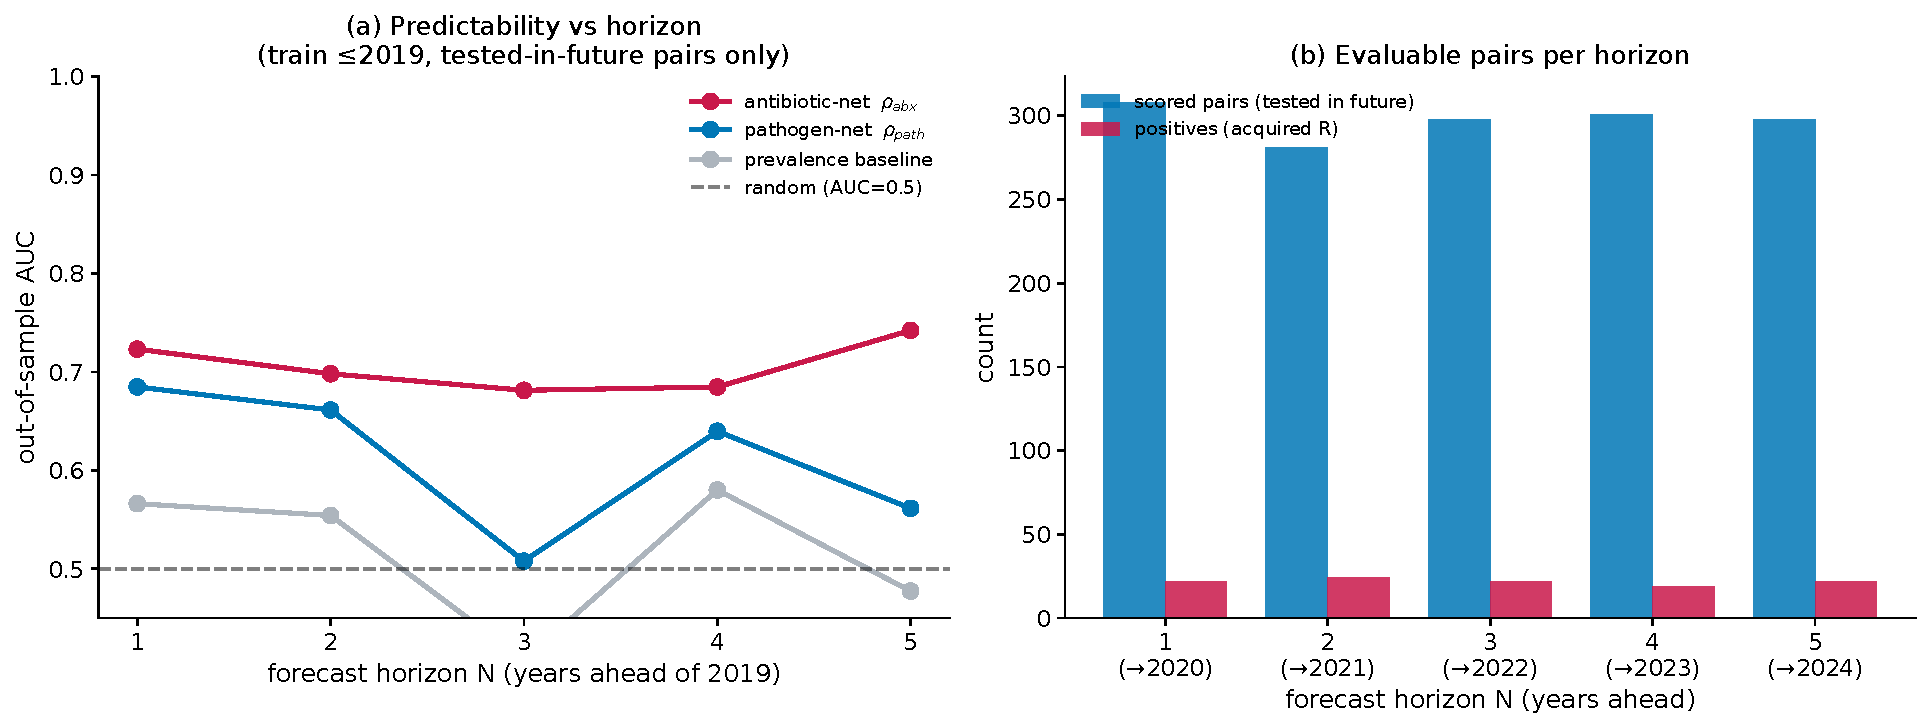
\includegraphics[width=\linewidth]{figures/fig6_horizon}
\caption{Multi-horizon forecasting from a single $t_0=2019$ cutoff. \textbf{(a)} Out-of-sample AUC
versus forecast horizon $N$: the antibiotic-network exposure $\rho_{abx}$ (red) stays at
$\sim\!0.7$ out to five years, well above the prevalence baseline (grey, near $0.5$), while the
pathogen-network score $\rho_{path}$ (blue) decays faster. \textbf{(b)} Number of evaluable pairs and
of realised positives per horizon, after dropping pairs untested in the target year.}
\label{fig:horizon}
\end{figure}

Finally, the horizon result is itself robust to the isolate threshold.
Table~\ref{tab:horizon-minN} repeats the multi-horizon sweep at $n_{\min}\in\{10,30,50\}$: the
antibiotic-network AUC averages $0.66$, $0.71$ and $0.72$ across the five horizons respectively, with
no systematic decay at any threshold. As in Appendix~\ref{app:minN}, the only visible effect is the
mild dilution of the signal at the permissive $n_{\min}=10$ setting; the paper's $n_{\min}=30$ and the
stricter $n_{\min}=50$ give essentially the same multi-year forecast.

\begin{table}[htbp]
\centering
\caption{Robustness of the multi-horizon forecast to $n_{\min}$: out-of-sample AUC of the
antibiotic-network exposure $\rho_{abx}$ at each horizon $N$ (train $\le 2019$). Predictability is flat
in $N$ at every threshold; the bottom row is the across-horizon mean.}
\label{tab:horizon-minN}
\small
\begin{tabular}{c ccc}
\toprule
 & \multicolumn{3}{c}{minimum isolates $n_{\min}$} \\
\cmidrule(lr){2-4}
Horizon $N$ (target) & $10$ & $30$ (paper) & $50$ \\
\midrule
1 (2020) & 0.596 & 0.723 & 0.715 \\
2 (2021) & 0.605 & 0.698 & 0.679 \\
3 (2022) & 0.728 & 0.681 & 0.741 \\
4 (2023) & 0.631 & 0.685 & 0.734 \\
5 (2024) & 0.715 & 0.742 & 0.723 \\
\midrule
mean     & 0.655 & 0.706 & 0.718 \\
\bottomrule
\end{tabular}
\end{table}

%  It reuses the main file's macros (\rca, \N, \I, \num) and the
%  booktabs / siunitx packages already loaded there.  The \providecommand
%  guards below let it also compile on its own if needed.
% =====================================================================
\providecommand{\rca}{\mathrm{RCA}}
\providecommand{\N}{\mathcal{N}}
\providecommand{\I}{\mathcal{I}}

\appendix

% ---------------------------------------------------------------------
\section{Robustness to the minimum-isolate threshold}
\label{app:minN}
% ---------------------------------------------------------------------
Every quantity in the paper is built from the pooled resistance-fraction matrix, in which a
species--antibiotic cell is retained only if it is supported by at least $n_{\min}$ tested isolates
in the pooling window. Throughout the main text we use $n_{\min}=30$: below this the resistance
fraction $r_{pa}=n_R/n_{\text{tested}}$ is too noisy to binarize reliably, while much above it the
matrix is thinned to the point where the within-block Spearman correlations lose power. To confirm
that no conclusion is an artefact of this single choice, we re-ran the \emph{entire} pipeline
(binarization, spectral co-clustering, nestedness, Fitness--Complexity, external validation and the
rolling-origin forecast) at $n_{\min}\in\{10,30,50\}$.\footnote{The threshold is the only quantity
changed. Note that the summary file distributed with the code
(\texttt{pathogen\_year\_antibiotic\_summary\_minN\_30.csv}) in fact contains \emph{all} cells down
to $n_{\text{tested}}=1$; the effective cut is applied in-code and is what we vary here. The file
name reflects the default rather than a pre-applied filter.}

Table~\ref{tab:minN-structure} reports the structural and external-validation statistics. All of the
paper's qualitative claims are preserved across the whole range: (i) global nestedness $\N$ sits at or
below the degree-preserving null while the in-block nestedness $\I^\ast$ is strongly significant
($z\ge 9.9$ everywhere), so nestedness remains a \emph{local}, block-level property with
$\I^\ast/\N$ between $5$ and $10$; (ii) antibiotic resistance complexity correlates positively with the
WHO AWaRe tier at every threshold, most strongly within blocks and within the Gram-negative block;
and (iii) in-block pathogen fitness separates ESKAPEE from non-ESKAPEE organisms with
$p\le 5\times10^{-6}$ throughout, while the corresponding \emph{global} fitness stays uninformative
(negative correlation with WHO priority), exactly the degeneracy the block analysis is meant to
expose. The AWaRe correlations peak at $n_{\min}=30$: relaxing to $10$ admits noisy low-count cells
that dilute them slightly, whereas tightening to $50$ removes enough antibiotics and species to cost
Spearman power (overall $\rho$ falls from $0.47$ to $0.35$). The default is thus a sensible optimum,
not a fragile edge.

\begin{table}[htbp]
\centering
\caption{Sensitivity of the structural and external-validation results to the minimum-isolate
threshold $n_{\min}$. The pooled window (2015--2024) and all other settings are held fixed;
$z$-scores are against \num{100} degree-preserving randomisations. Every conclusion in the main text
holds across the range; $n_{\min}=30$ (used in the paper) maximises the AWaRe correlations.}
\label{tab:minN-structure}
\small
\begin{tabular}{l ccc}
\toprule
 & \multicolumn{3}{c}{minimum isolates $n_{\min}$} \\
\cmidrule(lr){2-4}
Quantity & $10$ & $30$ (paper) & $50$ \\
\midrule
Resistant cells in $M$ (base rate)          & 191 (0.084) & 131 (0.071) & 99 (0.060) \\
\addlinespace[2pt]
Global nestedness $\N$ ($z$)                 & 0.073 ($-2.1$) & 0.050 ($-4.3$) & 0.039 ($-4.9$) \\
In-block nestedness $\I^\ast$ ($z$)          & 0.384 ($11.6$) & 0.386 ($10.5$) & 0.374 ($9.9$) \\
Ratio $\I^\ast/\N$                           & 5.3 & 7.8 & 9.6 \\
\addlinespace[2pt]
Complexity vs.\ AWaRe, overall $\rho$        & 0.434 & \textbf{0.467} & 0.347 \\
Complexity vs.\ AWaRe, in-block $\rho$       & 0.547 & \textbf{0.590} & 0.442 \\
Complexity vs.\ AWaRe, Gram-neg.\ $\rho$     & 0.613 & \textbf{0.624} & 0.546 \\
\addlinespace[2pt]
Global fitness vs.\ WHO priority $\rho$      & $-0.13$ & $-0.24$ & $-0.22$ \\
In-block fitness, ESKAPEE vs.\ non (median)  & $1.30$ / $-0.41$ & $1.04$ / $-0.39$ & $1.04$ / $-0.19$ \\
In-block fitness, ESKAPEE vs.\ non ($p$, MWU)& $2.4\times10^{-7}$ & $4.6\times10^{-6}$ & $5.6\times10^{-7}$ \\
\bottomrule
\end{tabular}
\end{table}

Table~\ref{tab:minN-forecast} shows the same insensitivity for the headline rolling-origin forecast
(2020--2024). The network-exposure score $\rho_{abx}$ beats the resistance-prevalence baseline at
every threshold. The forecast is essentially unchanged between $n_{\min}=30$ and $50$
(AUC $0.708$ vs.\ $0.702$); only the permissive $n_{\min}=10$ setting degrades it appreciably
(AUC $0.638$), because the extra low-count cells inject label noise into exactly the pairs the
predictor is scored on. The prevalence baseline stays near chance throughout, confirming that the
predictive signal comes from network structure rather than from base rates.

\begin{table}[htbp]
\centering
\caption{Sensitivity of the pooled rolling-origin forecast (origins $2019\ldots2023$, predicting
$2020\ldots2024$) to $n_{\min}$. AUC is the rank-based area under the ROC on the pooled candidate set;
the co-resistance exposure $\rho_{abx}$ dominates the prevalence baseline at every threshold.}
\label{tab:minN-forecast}
\small
\begin{tabular}{l ccc}
\toprule
 & \multicolumn{3}{c}{minimum isolates $n_{\min}$} \\
\cmidrule(lr){2-4}
 & $10$ & $30$ (paper) & $50$ \\
\midrule
Candidate pairs (positives)               & 2274 (191) & 1839 (131) & 1656 (99) \\
Base rate                                 & 0.084 & 0.071 & 0.060 \\
\addlinespace[2pt]
AUC, antibiotic-net $\rho_{abx}$          & 0.638 & \textbf{0.708} & 0.702 \\
AUC, pathogen-net $\rho_{path}$           & 0.622 & 0.628 & 0.593 \\
AUC, prevalence baseline                  & 0.544 & 0.512 & 0.504 \\
\bottomrule
\end{tabular}
\end{table}

% ---------------------------------------------------------------------
\section{Multi-year (multi-horizon) forecasting}
\label{app:horizon}
% ---------------------------------------------------------------------
The rolling-origin test in the main text always predicts one year ahead ($t\to t+1$). A natural
question is how far into the future the co-resistance signal reaches. To isolate the pure effect of
forecast \emph{distance} we fix a single training cutoff $t_0=2019$, build the binary matrix, the
co-resistance projection $W$ and every exposure feature $\rho_{pa}$ \emph{once} from data with
year $\le t_0$, and then score that one frozen model against each future target year $t_0+N$ for
$N=1,\ldots,5$ (i.e.\ 2020 through 2024). The training history, the network and the candidate set are
identical for every horizon; only the target year moves, so any change in AUC is attributable to
forecast distance alone and not to a re-fitted model.

We additionally require that a candidate pathogen--antibiotic pair be \emph{actually tested}
($n_{\text{tested}}\ge n_{\min}$) in the future target year: a predicted pair with no measurement in
$t_0+N$ has no ground truth and is dropped rather than silently counted as a negative. About two
thirds of the frozen candidate set is dropped this way at each horizon (roughly $35\%$ retained),
which is reported alongside the AUC so the shrinking evaluable sample is explicit.

Table~\ref{tab:horizon} gives the result at the paper's $n_{\min}=30$ and is plotted in
Fig.~\ref{fig:horizon}. The striking finding is that predictability does \emph{not} decay with
horizon over this window: the antibiotic-network exposure holds an AUC of $0.68$--$0.74$ all the way
out to five years, with no monotone fall-off, while the prevalence baseline hovers near chance
($0.41$--$0.58$) at every distance. In other words, the structural co-resistance signal identified in
the main text is not a short-lived, next-year-only effect; the pairs a pathogen is network-``exposed''
to remain the pairs it tends to acquire years later. The pathogen-network score $\rho_{path}$ is
weaker and noisier at long range (falling toward $0.5$ by $N=3$), consistent with the main-text
finding that the antibiotic-side projection carries most of the predictive information.

\begin{table}[htbp]
\centering
\caption{Single-cutoff multi-horizon forecast, trained once on $2004$--$2019$ and evaluated on each
future year, restricted to pairs tested in that year ($n_{\min}=30$). Predictability is roughly flat
out to five years; the prevalence baseline stays near chance throughout.}
\label{tab:horizon}
\small
\begin{tabular}{c c cc ccc}
\toprule
Horizon $N$ & Target & Tested pairs & Positives (rate) & AUC $\rho_{abx}$ & AUC $\rho_{path}$ & AUC prevalence \\
\midrule
1 & 2020 & 308 & 22 (0.071) & 0.723 & 0.685 & 0.566 \\
2 & 2021 & 281 & 24 (0.085) & 0.698 & 0.661 & 0.554 \\
3 & 2022 & 298 & 22 (0.074) & 0.681 & 0.508 & 0.407 \\
4 & 2023 & 301 & 19 (0.063) & 0.685 & 0.640 & 0.580 \\
5 & 2024 & 298 & 22 (0.074) & 0.742 & 0.561 & 0.477 \\
\bottomrule
\end{tabular}
\end{table}

\begin{figure}[htbp]
\centering
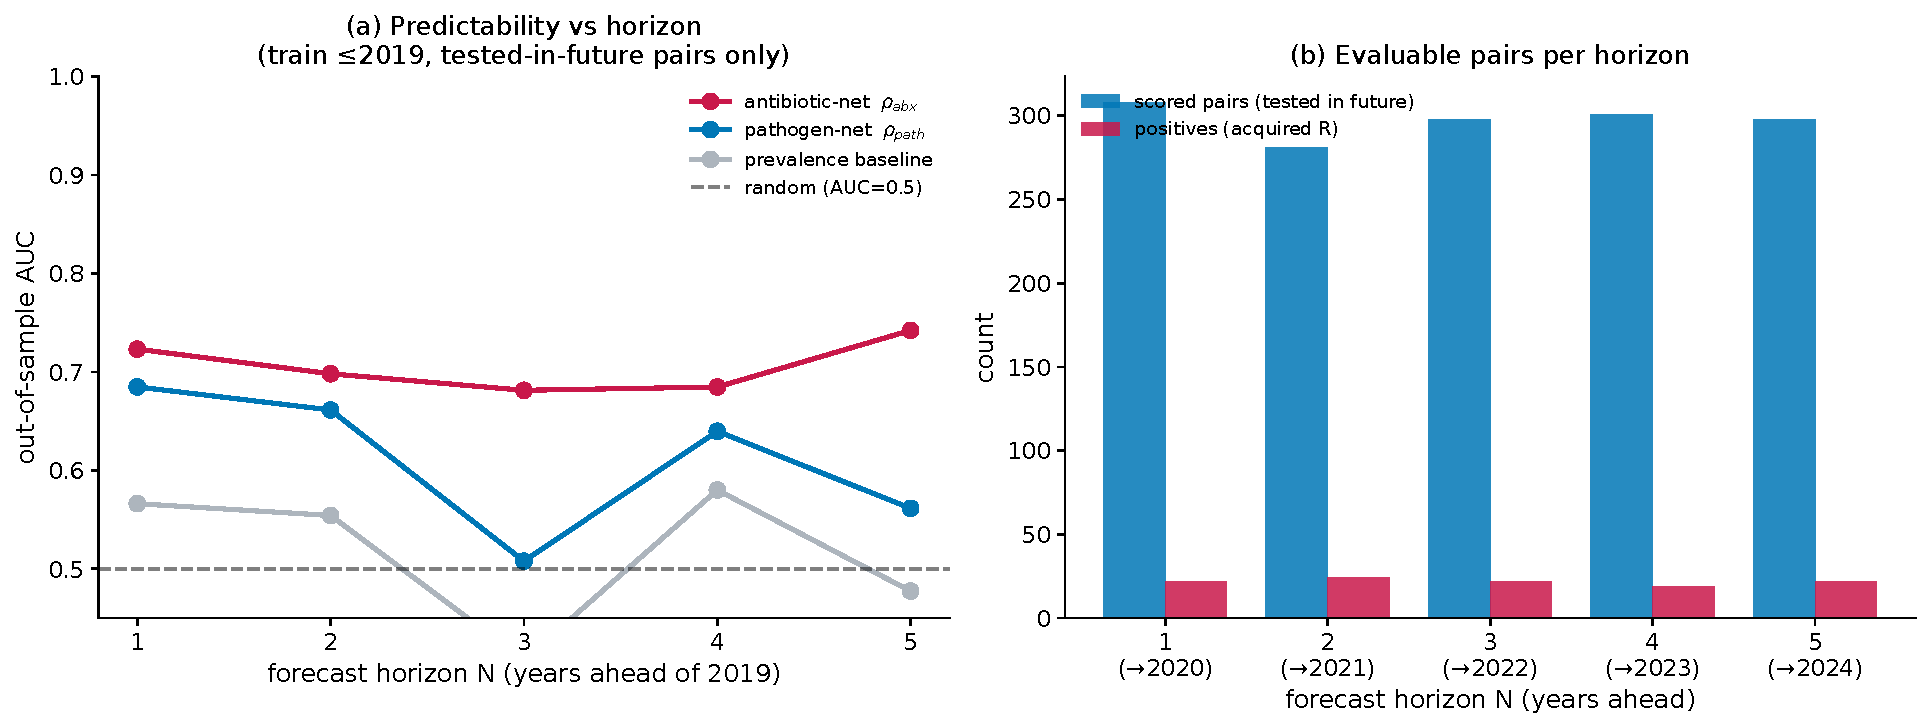
\includegraphics[width=\linewidth]{figures/fig6_horizon}
\caption{Multi-horizon forecasting from a single $t_0=2019$ cutoff. \textbf{(a)} Out-of-sample AUC
versus forecast horizon $N$: the antibiotic-network exposure $\rho_{abx}$ (red) stays at
$\sim\!0.7$ out to five years, well above the prevalence baseline (grey, near $0.5$), while the
pathogen-network score $\rho_{path}$ (blue) decays faster. \textbf{(b)} Number of evaluable pairs and
of realised positives per horizon, after dropping pairs untested in the target year.}
\label{fig:horizon}
\end{figure}

Finally, the horizon result is itself robust to the isolate threshold.
Table~\ref{tab:horizon-minN} repeats the multi-horizon sweep at $n_{\min}\in\{10,30,50\}$: the
antibiotic-network AUC averages $0.66$, $0.71$ and $0.72$ across the five horizons respectively, with
no systematic decay at any threshold. As in Appendix~\ref{app:minN}, the only visible effect is the
mild dilution of the signal at the permissive $n_{\min}=10$ setting; the paper's $n_{\min}=30$ and the
stricter $n_{\min}=50$ give essentially the same multi-year forecast.

\begin{table}[htbp]
\centering
\caption{Robustness of the multi-horizon forecast to $n_{\min}$: out-of-sample AUC of the
antibiotic-network exposure $\rho_{abx}$ at each horizon $N$ (train $\le 2019$). Predictability is flat
in $N$ at every threshold; the bottom row is the across-horizon mean.}
\label{tab:horizon-minN}
\small
\begin{tabular}{c ccc}
\toprule
 & \multicolumn{3}{c}{minimum isolates $n_{\min}$} \\
\cmidrule(lr){2-4}
Horizon $N$ (target) & $10$ & $30$ (paper) & $50$ \\
\midrule
1 (2020) & 0.596 & 0.723 & 0.715 \\
2 (2021) & 0.605 & 0.698 & 0.679 \\
3 (2022) & 0.728 & 0.681 & 0.741 \\
4 (2023) & 0.631 & 0.685 & 0.734 \\
5 (2024) & 0.715 & 0.742 & 0.723 \\
\midrule
mean     & 0.655 & 0.706 & 0.718 \\
\bottomrule
\end{tabular}
\end{table}

%  It reuses the main file's macros (\rca, \N, \I, \num) and the
%  booktabs / siunitx packages already loaded there.  The \providecommand
%  guards below let it also compile on its own if needed.
% =====================================================================
\providecommand{\rca}{\mathrm{RCA}}
\providecommand{\N}{\mathcal{N}}
\providecommand{\I}{\mathcal{I}}

\appendix

% ---------------------------------------------------------------------
\section{Robustness to the minimum-isolate threshold}
\label{app:minN}
% ---------------------------------------------------------------------
Every quantity in the paper is built from the pooled resistance-fraction matrix, in which a
species--antibiotic cell is retained only if it is supported by at least $n_{\min}$ tested isolates
in the pooling window. Throughout the main text we use $n_{\min}=30$: below this the resistance
fraction $r_{pa}=n_R/n_{\text{tested}}$ is too noisy to binarize reliably, while much above it the
matrix is thinned to the point where the within-block Spearman correlations lose power. To confirm
that no conclusion is an artefact of this single choice, we re-ran the \emph{entire} pipeline
(binarization, spectral co-clustering, nestedness, Fitness--Complexity, external validation and the
rolling-origin forecast) at $n_{\min}\in\{10,30,50\}$.\footnote{The threshold is the only quantity
changed. Note that the summary file distributed with the code
(\texttt{pathogen\_year\_antibiotic\_summary\_minN\_30.csv}) in fact contains \emph{all} cells down
to $n_{\text{tested}}=1$; the effective cut is applied in-code and is what we vary here. The file
name reflects the default rather than a pre-applied filter.}

Table~\ref{tab:minN-structure} reports the structural and external-validation statistics. All of the
paper's qualitative claims are preserved across the whole range: (i) global nestedness $\N$ sits at or
below the degree-preserving null while the in-block nestedness $\I^\ast$ is strongly significant
($z\ge 9.9$ everywhere), so nestedness remains a \emph{local}, block-level property with
$\I^\ast/\N$ between $5$ and $10$; (ii) antibiotic resistance complexity correlates positively with the
WHO AWaRe tier at every threshold, most strongly within blocks and within the Gram-negative block;
and (iii) in-block pathogen fitness separates ESKAPEE from non-ESKAPEE organisms with
$p\le 5\times10^{-6}$ throughout, while the corresponding \emph{global} fitness stays uninformative
(negative correlation with WHO priority), exactly the degeneracy the block analysis is meant to
expose. The AWaRe correlations peak at $n_{\min}=30$: relaxing to $10$ admits noisy low-count cells
that dilute them slightly, whereas tightening to $50$ removes enough antibiotics and species to cost
Spearman power (overall $\rho$ falls from $0.47$ to $0.35$). The default is thus a sensible optimum,
not a fragile edge.

\begin{table}[htbp]
\centering
\caption{Sensitivity of the structural and external-validation results to the minimum-isolate
threshold $n_{\min}$. The pooled window (2015--2024) and all other settings are held fixed;
$z$-scores are against \num{100} degree-preserving randomisations. Every conclusion in the main text
holds across the range; $n_{\min}=30$ (used in the paper) maximises the AWaRe correlations.}
\label{tab:minN-structure}
\small
\begin{tabular}{l ccc}
\toprule
 & \multicolumn{3}{c}{minimum isolates $n_{\min}$} \\
\cmidrule(lr){2-4}
Quantity & $10$ & $30$ (paper) & $50$ \\
\midrule
Resistant cells in $M$ (base rate)          & 191 (0.084) & 131 (0.071) & 99 (0.060) \\
\addlinespace[2pt]
Global nestedness $\N$ ($z$)                 & 0.073 ($-2.1$) & 0.050 ($-4.3$) & 0.039 ($-4.9$) \\
In-block nestedness $\I^\ast$ ($z$)          & 0.384 ($11.6$) & 0.386 ($10.5$) & 0.374 ($9.9$) \\
Ratio $\I^\ast/\N$                           & 5.3 & 7.8 & 9.6 \\
\addlinespace[2pt]
Complexity vs.\ AWaRe, overall $\rho$        & 0.434 & \textbf{0.467} & 0.347 \\
Complexity vs.\ AWaRe, in-block $\rho$       & 0.547 & \textbf{0.590} & 0.442 \\
Complexity vs.\ AWaRe, Gram-neg.\ $\rho$     & 0.613 & \textbf{0.624} & 0.546 \\
\addlinespace[2pt]
Global fitness vs.\ WHO priority $\rho$      & $-0.13$ & $-0.24$ & $-0.22$ \\
In-block fitness, ESKAPEE vs.\ non (median)  & $1.30$ / $-0.41$ & $1.04$ / $-0.39$ & $1.04$ / $-0.19$ \\
In-block fitness, ESKAPEE vs.\ non ($p$, MWU)& $2.4\times10^{-7}$ & $4.6\times10^{-6}$ & $5.6\times10^{-7}$ \\
\bottomrule
\end{tabular}
\end{table}

Table~\ref{tab:minN-forecast} shows the same insensitivity for the headline rolling-origin forecast
(2020--2024). The network-exposure score $\rho_{abx}$ beats the resistance-prevalence baseline at
every threshold. The forecast is essentially unchanged between $n_{\min}=30$ and $50$
(AUC $0.708$ vs.\ $0.702$); only the permissive $n_{\min}=10$ setting degrades it appreciably
(AUC $0.638$), because the extra low-count cells inject label noise into exactly the pairs the
predictor is scored on. The prevalence baseline stays near chance throughout, confirming that the
predictive signal comes from network structure rather than from base rates.

\begin{table}[htbp]
\centering
\caption{Sensitivity of the pooled rolling-origin forecast (origins $2019\ldots2023$, predicting
$2020\ldots2024$) to $n_{\min}$. AUC is the rank-based area under the ROC on the pooled candidate set;
the co-resistance exposure $\rho_{abx}$ dominates the prevalence baseline at every threshold.}
\label{tab:minN-forecast}
\small
\begin{tabular}{l ccc}
\toprule
 & \multicolumn{3}{c}{minimum isolates $n_{\min}$} \\
\cmidrule(lr){2-4}
 & $10$ & $30$ (paper) & $50$ \\
\midrule
Candidate pairs (positives)               & 2274 (191) & 1839 (131) & 1656 (99) \\
Base rate                                 & 0.084 & 0.071 & 0.060 \\
\addlinespace[2pt]
AUC, antibiotic-net $\rho_{abx}$          & 0.638 & \textbf{0.708} & 0.702 \\
AUC, pathogen-net $\rho_{path}$           & 0.622 & 0.628 & 0.593 \\
AUC, prevalence baseline                  & 0.544 & 0.512 & 0.504 \\
\bottomrule
\end{tabular}
\end{table}

% ---------------------------------------------------------------------
\section{Multi-year (multi-horizon) forecasting}
\label{app:horizon}
% ---------------------------------------------------------------------
The rolling-origin test in the main text always predicts one year ahead ($t\to t+1$). A natural
question is how far into the future the co-resistance signal reaches. To isolate the pure effect of
forecast \emph{distance} we fix a single training cutoff $t_0=2019$, build the binary matrix, the
co-resistance projection $W$ and every exposure feature $\rho_{pa}$ \emph{once} from data with
year $\le t_0$, and then score that one frozen model against each future target year $t_0+N$ for
$N=1,\ldots,5$ (i.e.\ 2020 through 2024). The training history, the network and the candidate set are
identical for every horizon; only the target year moves, so any change in AUC is attributable to
forecast distance alone and not to a re-fitted model.

We additionally require that a candidate pathogen--antibiotic pair be \emph{actually tested}
($n_{\text{tested}}\ge n_{\min}$) in the future target year: a predicted pair with no measurement in
$t_0+N$ has no ground truth and is dropped rather than silently counted as a negative. About two
thirds of the frozen candidate set is dropped this way at each horizon (roughly $35\%$ retained),
which is reported alongside the AUC so the shrinking evaluable sample is explicit.

Table~\ref{tab:horizon} gives the result at the paper's $n_{\min}=30$ and is plotted in
Fig.~\ref{fig:horizon}. The striking finding is that predictability does \emph{not} decay with
horizon over this window: the antibiotic-network exposure holds an AUC of $0.68$--$0.74$ all the way
out to five years, with no monotone fall-off, while the prevalence baseline hovers near chance
($0.41$--$0.58$) at every distance. In other words, the structural co-resistance signal identified in
the main text is not a short-lived, next-year-only effect; the pairs a pathogen is network-``exposed''
to remain the pairs it tends to acquire years later. The pathogen-network score $\rho_{path}$ is
weaker and noisier at long range (falling toward $0.5$ by $N=3$), consistent with the main-text
finding that the antibiotic-side projection carries most of the predictive information.

\begin{table}[htbp]
\centering
\caption{Single-cutoff multi-horizon forecast, trained once on $2004$--$2019$ and evaluated on each
future year, restricted to pairs tested in that year ($n_{\min}=30$). Predictability is roughly flat
out to five years; the prevalence baseline stays near chance throughout.}
\label{tab:horizon}
\small
\begin{tabular}{c c cc ccc}
\toprule
Horizon $N$ & Target & Tested pairs & Positives (rate) & AUC $\rho_{abx}$ & AUC $\rho_{path}$ & AUC prevalence \\
\midrule
1 & 2020 & 308 & 22 (0.071) & 0.723 & 0.685 & 0.566 \\
2 & 2021 & 281 & 24 (0.085) & 0.698 & 0.661 & 0.554 \\
3 & 2022 & 298 & 22 (0.074) & 0.681 & 0.508 & 0.407 \\
4 & 2023 & 301 & 19 (0.063) & 0.685 & 0.640 & 0.580 \\
5 & 2024 & 298 & 22 (0.074) & 0.742 & 0.561 & 0.477 \\
\bottomrule
\end{tabular}
\end{table}

\begin{figure}[htbp]
\centering
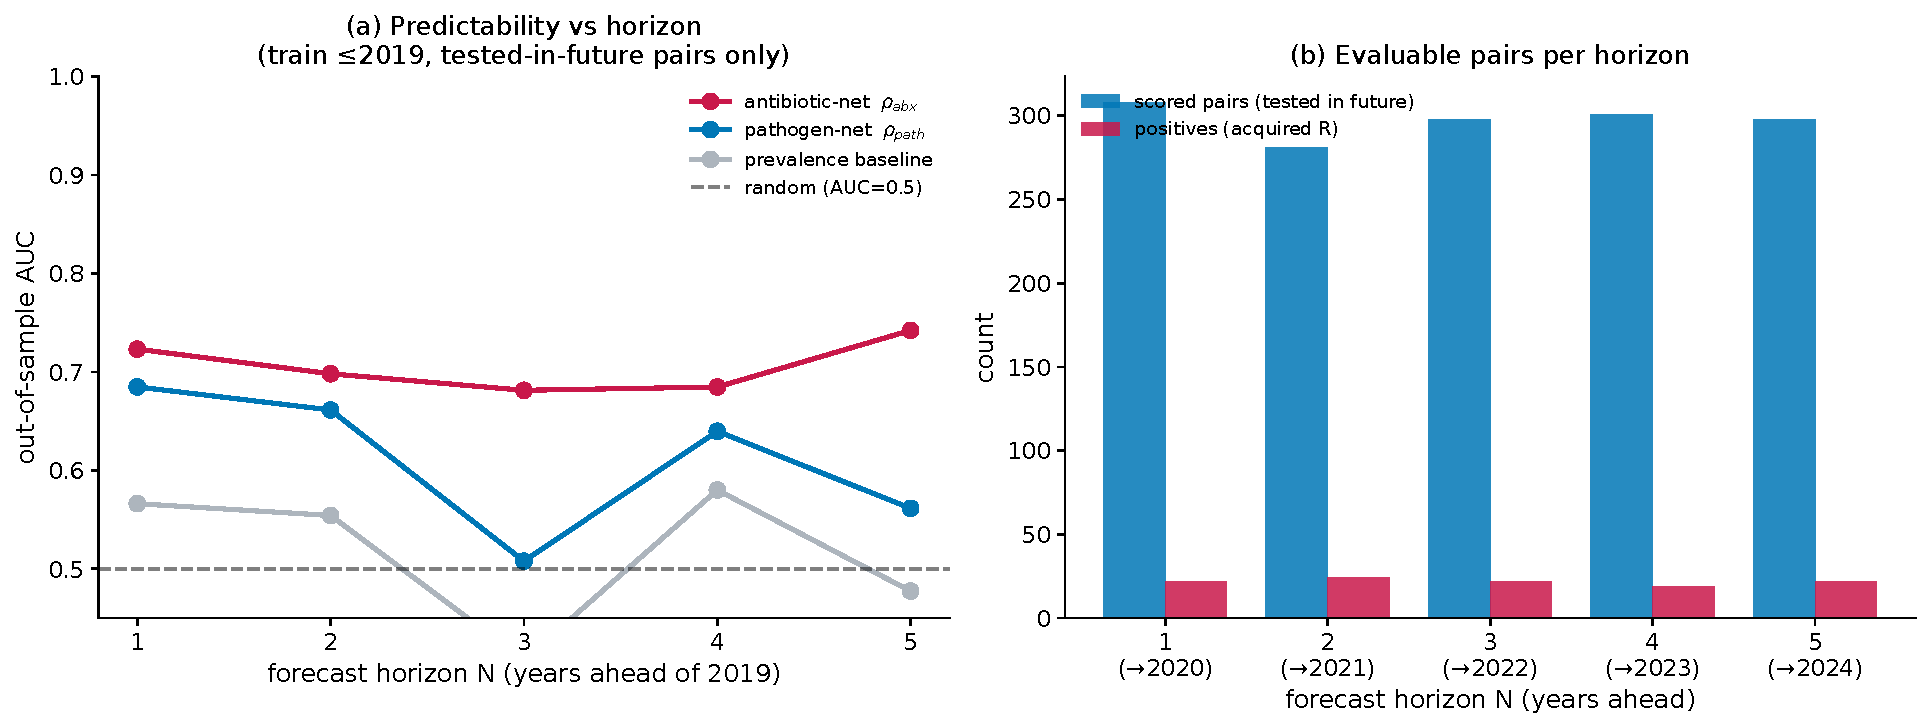
\includegraphics[width=\linewidth]{figures/fig6_horizon}
\caption{Multi-horizon forecasting from a single $t_0=2019$ cutoff. \textbf{(a)} Out-of-sample AUC
versus forecast horizon $N$: the antibiotic-network exposure $\rho_{abx}$ (red) stays at
$\sim\!0.7$ out to five years, well above the prevalence baseline (grey, near $0.5$), while the
pathogen-network score $\rho_{path}$ (blue) decays faster. \textbf{(b)} Number of evaluable pairs and
of realised positives per horizon, after dropping pairs untested in the target year.}
\label{fig:horizon}
\end{figure}

Finally, the horizon result is itself robust to the isolate threshold.
Table~\ref{tab:horizon-minN} repeats the multi-horizon sweep at $n_{\min}\in\{10,30,50\}$: the
antibiotic-network AUC averages $0.66$, $0.71$ and $0.72$ across the five horizons respectively, with
no systematic decay at any threshold. As in Appendix~\ref{app:minN}, the only visible effect is the
mild dilution of the signal at the permissive $n_{\min}=10$ setting; the paper's $n_{\min}=30$ and the
stricter $n_{\min}=50$ give essentially the same multi-year forecast.

\begin{table}[htbp]
\centering
\caption{Robustness of the multi-horizon forecast to $n_{\min}$: out-of-sample AUC of the
antibiotic-network exposure $\rho_{abx}$ at each horizon $N$ (train $\le 2019$). Predictability is flat
in $N$ at every threshold; the bottom row is the across-horizon mean.}
\label{tab:horizon-minN}
\small
\begin{tabular}{c ccc}
\toprule
 & \multicolumn{3}{c}{minimum isolates $n_{\min}$} \\
\cmidrule(lr){2-4}
Horizon $N$ (target) & $10$ & $30$ (paper) & $50$ \\
\midrule
1 (2020) & 0.596 & 0.723 & 0.715 \\
2 (2021) & 0.605 & 0.698 & 0.679 \\
3 (2022) & 0.728 & 0.681 & 0.741 \\
4 (2023) & 0.631 & 0.685 & 0.734 \\
5 (2024) & 0.715 & 0.742 & 0.723 \\
\midrule
mean     & 0.655 & 0.706 & 0.718 \\
\bottomrule
\end{tabular}
\end{table}
